\documentclass{report}
\usepackage[utf8]{inputenc}
\usepackage[T1]{fontenc}
\usepackage{graphicx} 
\usepackage{amsmath}
\usepackage{float} 
\usepackage[parfill]{parskip} 
\widowpenalty=10000
\clubpenalty=10000

\title{Longitudinal Analysis of Nepals's Performance and Selection System in Mathematics Olympiad Circuit}
\author{Hridam Adhikari}
\date{March 2026}

\begin{document}

\maketitle

\begin{abstract}
This paper analyzes Nepal's International Mathematical Olympiad journey from 2017 to 2025, with particular focus on whether internal selection tests, the Pre-Team Selection test(PTST) and Team Selection Test (TST), serve as reliable predictors of international performance. Using publicly available data from Mathematics Association of Nepal (MAN) for three complete selection cycles(2023, 2024 and 2025), this paper aims to evaluate the predictive validity of internal tests, identify question biases, and present Nepal's growth at the IMO. The findings reveal that while neither PTST nor TST accurately predicts the absolute IMO scores, the TST demonstrates moderate ability to predict relative trends and rankings among the team members. Furthermore, a structural bias towards easier problems(P1/P4 problems) in internal testing examinations (TST and PTST) is identified as the likely the primary driver of Nepal's recent accelerating growth at the IMO. However, this trend suggests the possibility for a performance plateau if the internal testing strategies aren’t changed. The paper concludes with recommendation focusing on improving testing strategies for long-term growth.
\end{abstract}

\section{Introduction}
Nepal initiated participation in International Mathematical Olympiad in 2017. Since then, Nepal has shown a gradual growth in terms of the performance, with the recent IMO held in Sunshine Coast, Australia, representing the most successful outcome till date. (A candidate was able to secure bronze medal, highest feat for the country in IMO). Alongside this, the candidates have received multiple Honorable mention awards over the years, suggesting the rise of mathematical competency among the national cohort. 

Despite this progress, the internal testing mechanisms based on which candidates are selected for the international event remains largely unevaluated. The testing system consists of multiple stages starting from district level to provincial level to national level followed by Pre-Team Selection Test, Closed Camp, and Team Selection Test.

\section{Objectives}
The paper contains four major objectives: 

\begin{itemize}
    \item[I)] To examine if the internal tests (PTST and TST) predict IMO scores, in terms of numerical marks and relative rankings.
    \item[II)] To analyze the marks received by the candidates on the basis of question types based on difficulty, where P1 and P4 are classified easiest, P2 and P5 as medium, and P3 and P6 as hardest of them all.
    \item[III)] To identify Nepal's growth in IMO and assess its long-term sustainability.
\end{itemize}
\newpage
\section{Methodology}

\subsection{Division I: Longitudinal IMO Performance Assessment(2017-2025)}
Official IMO data were collected from the IMO database for all the years that Nepal has participated i.e. from 2017 to 2025. The data were then structured in CSV format for analysis and merged for proper comparison. The data frame was then visualized as line graphs and pie charts to identify trend and pattern across all seven years. The code for this part was written to prioritize reusability so that any future year's data can be appended with minimal modification.

\subsection{Division II: Internal Testing Assessment(Data from 2023 to 2025)}
Internal Testing Data for the years 2023, 2024 and 2025 were sourced from the results published by Mathematical Association in Nepal (The organization which looks after Math Olympiads in Nepal). These data were then structured into CSV format and pre-processed using the Pandas library in Python. After that, a reproducible computational workflow was implemented using Python. This workflow involved data selection, extraction, cleaning, normalization and merging datasets. The process was then followed by data visualization which was done with the Matplotlib's pyplot module. The task was done in the Jupyter notebook to ensure that the comments were embedded throughout the codes. 

\subsection{Key Methodology Principles}

\begin{itemize}
    \item[I)] Conclusions were drawn only when the pattern was consistent across multiple datasets.
    \item[ii)] All the scores (from PTST and TST) were converted to a scale of 42 matching the scale of IMO to enable fair cross-test comparison.
    \item[iii)] The datasets were managed in such a way that they returned patterns which fulfilled the objective of the project.
    \item[iv)] The comparisons focus on trends and relative rankings in addition to raw marks as the small data size (6 per year) means that the numerical comparisons may not be reliable.
\end{itemize}
\newpage
\section{Findings and Analysis}
\label{sec:findings}

\subsection{Nepal's IMO Trajectory}

Figure \ref{fig1} presents the contribution of each year from 2017 to 2025 in Nepal's cumulative IMO score.

\begin{figure}[H] 
    \centering
    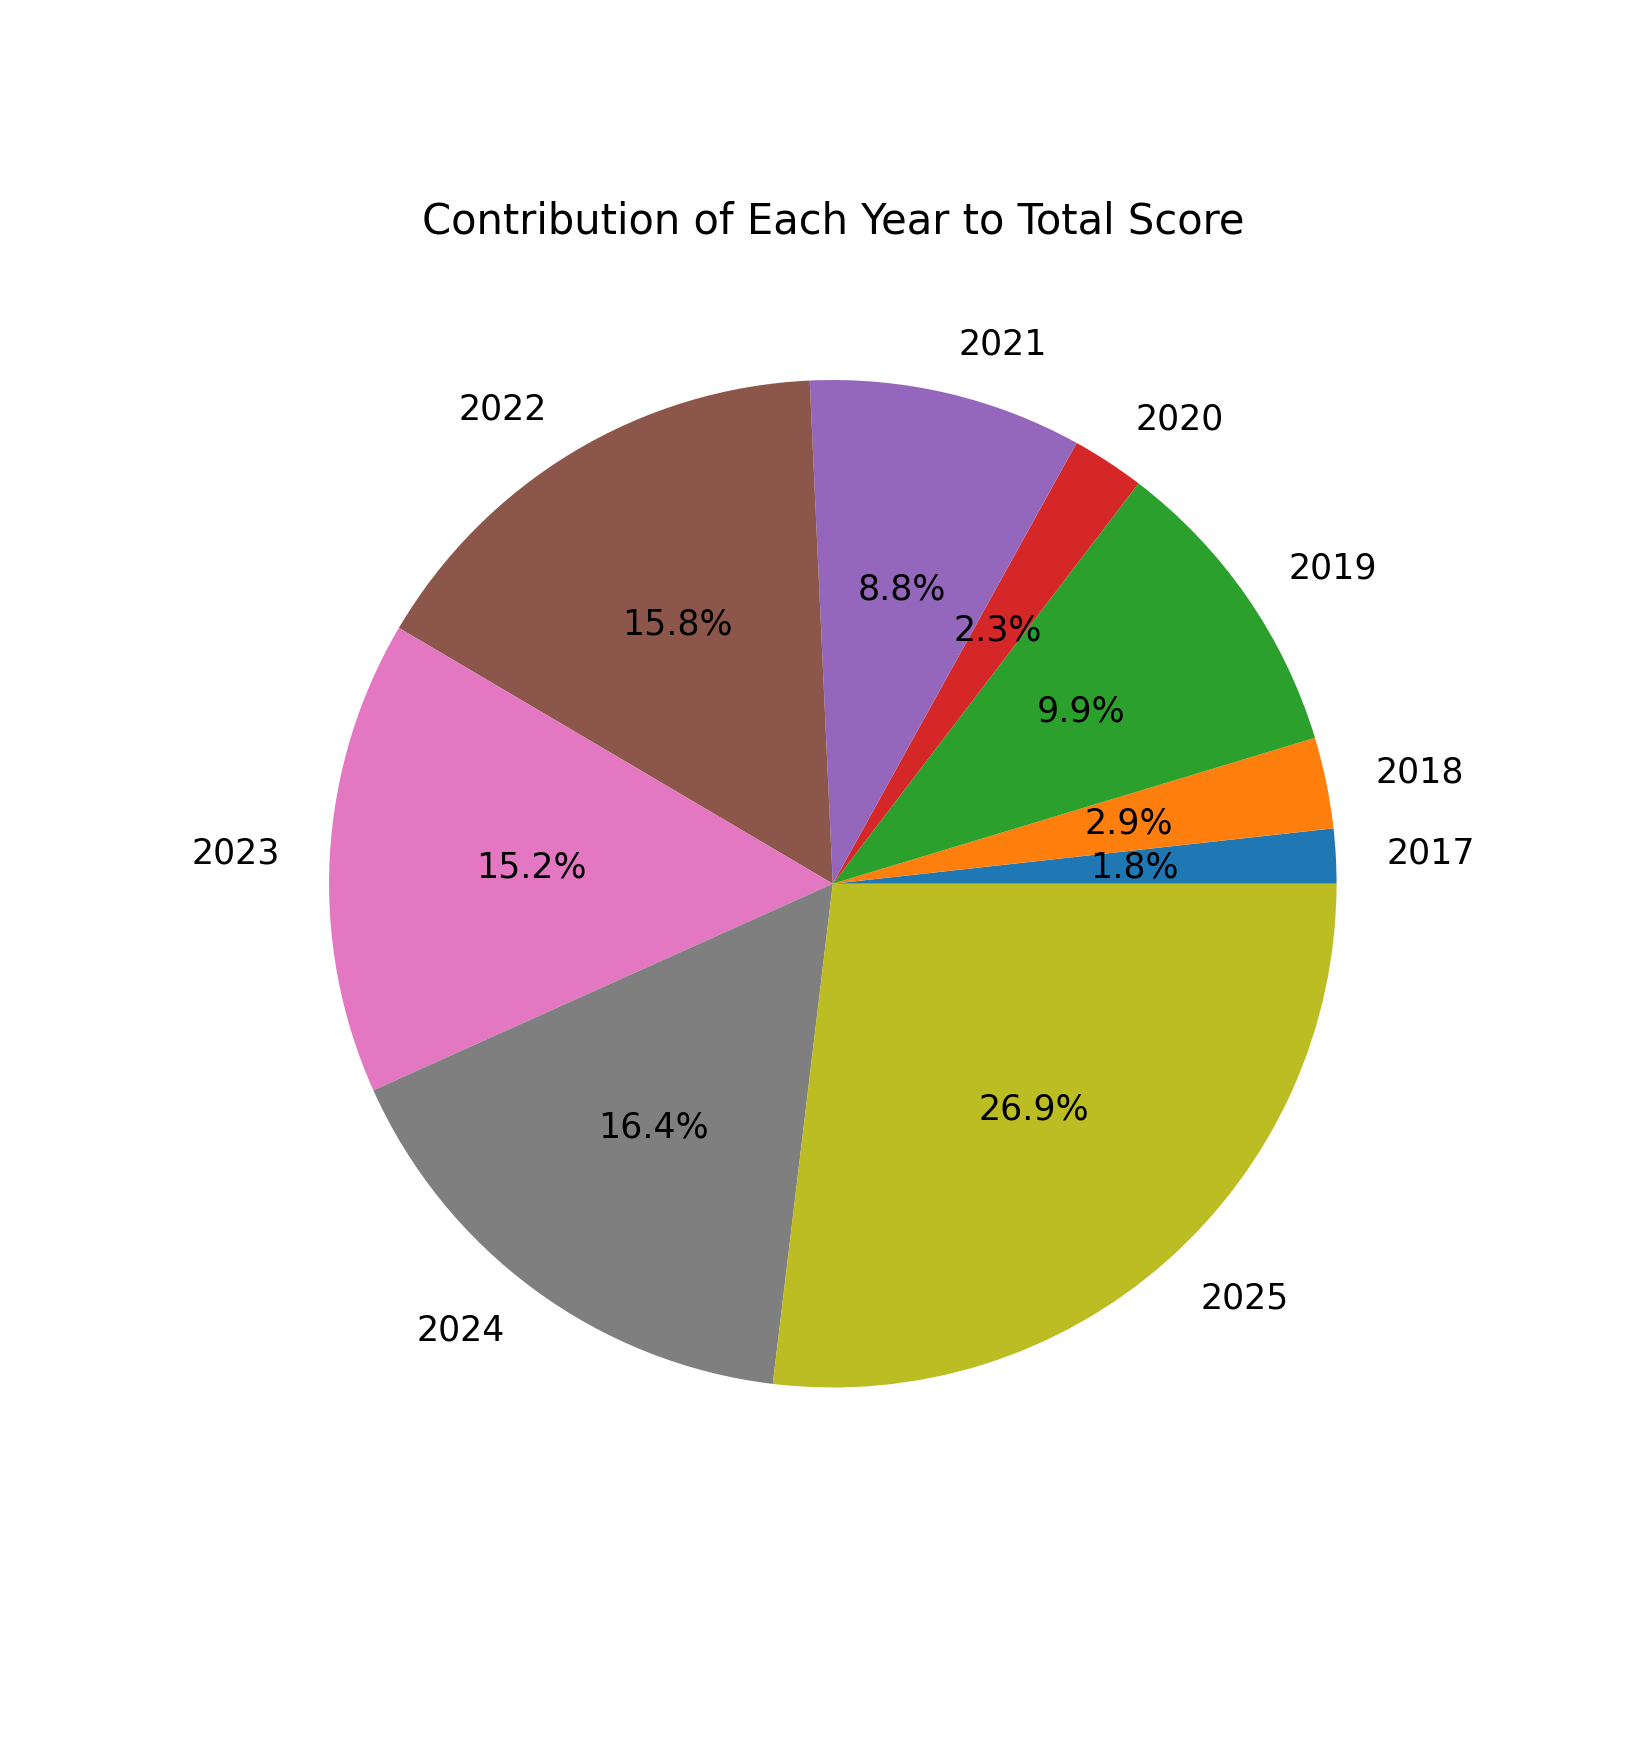
\includegraphics[width=0.5\textwidth]{total_scores_pie.png}
    \caption{Contribution of each year from 2017 to 2025 to Nepal's total cumulative IMO score.}
    \label{fig1}
\end{figure}

The data suggests that Nepal's growth at the International Mathematics Olympiad has been rapid and accelerating in recent years, with earlier years showing a slower and more inconsistent trend. The years from 2022 to 2025 account for nearly 74\% of the total marks attained, with recent IMO in Sunshine coast, Australia contributing 26.9\%. This pattern shows signs of critical mass effect, where after having a slow start due to the growth of institutional knowledge and higher training data the country is experiencing growth in a rapid rate. 

However, this pie chart alone cannot reveal whether this growth is broad or concentrated. The following sections will visualize this clearly.

\subsection{Problem Level Performance}
The Figure \ref{fig2} and \ref{fig3} illustrate the problem wise performance of Nepal in International Mathematics Olympiad. Here the questions are separated into two graphs, where P1-P3 is in the first graph while P4-P6 is in the second graph. In IMO, the questions are numbered on the basis of their difficulty where P1/P4 are the easiest, P2/P5 are medium, and P3/P6 are the hardest. 
\newpage
\begin{figure}[H]
    \centering
    \includegraphics[width=0.6\textwidth]{year1_3.png}
    \caption{The problem wise marks for questions P1-P3 (P1: Blue, P2: Yellow, P3: Green), from the year 2017 to 2025.}
    \label{fig2}
\end{figure}

\begin{figure}[H]
    \centering
    \includegraphics[width=0.6\textwidth]{year4_6.png}
    \caption{The problem wise marks for questions P4-P6 (P4: Blue, P5: Yellow, P6: Green), from the year 2017 to 2025.}
    \label{fig3}
\end{figure}

There are some patterns across both the figures which will help us with our objective:

\begin{itemize}
    \item[i)] P3 and P6 (two hardest problems in IMO) have never been solved by any Nepal team member with combined score of just 1 across 9 years of participation.
    \item[ii)] P1 and P4 (two easier problems in IMO) have had a steady growth and account for large majority of Nepal's total IMO score in recent years. 
    \item[iii)] P2 and P5 provide occasional improvement (spikes) in the chart, however the spikes are very inconsistent to show any sort of trend. 
\end{itemize}

The steep rise in P4 scores is particularly significant. From near zero in 2017-2020, the team collected 25 total points in P4. The rise in marks collected from P1 is clear as well. This reflects a developing mastery of P1/P4 type questions among the test takers, which is an incredible feat as it's slowly mounting up the total scores. However, the inconsistent performance in P2 and P5 and flat lines for P3 and P6 signals concern. While Nepal's students seem to have developed their skills in easy end of problem spectrum, they are yet to break through in medium and hard questions. 

Finding: Nepal's growth in IMO seems to be concentrated in narrow band of problem difficulty.

\subsection{Score Distributions( Mean and Standard deviation)}
\label{sec:distributions}
Recognizing the P1/P4 pattern at international level, we need to examine if internal testing system reflects and additionally reinforces such pattern to draw out recommendations. In this section, mean and standard deviation for internal testing across three years are examined. The Figure \ref{fig4}, \ref{fig5} and \ref{fig6} show the mean scores for PTST, TST and IMO for the years 2023, 2024, and 2025 respectively. 

\begin{figure}[H]
    \centering
    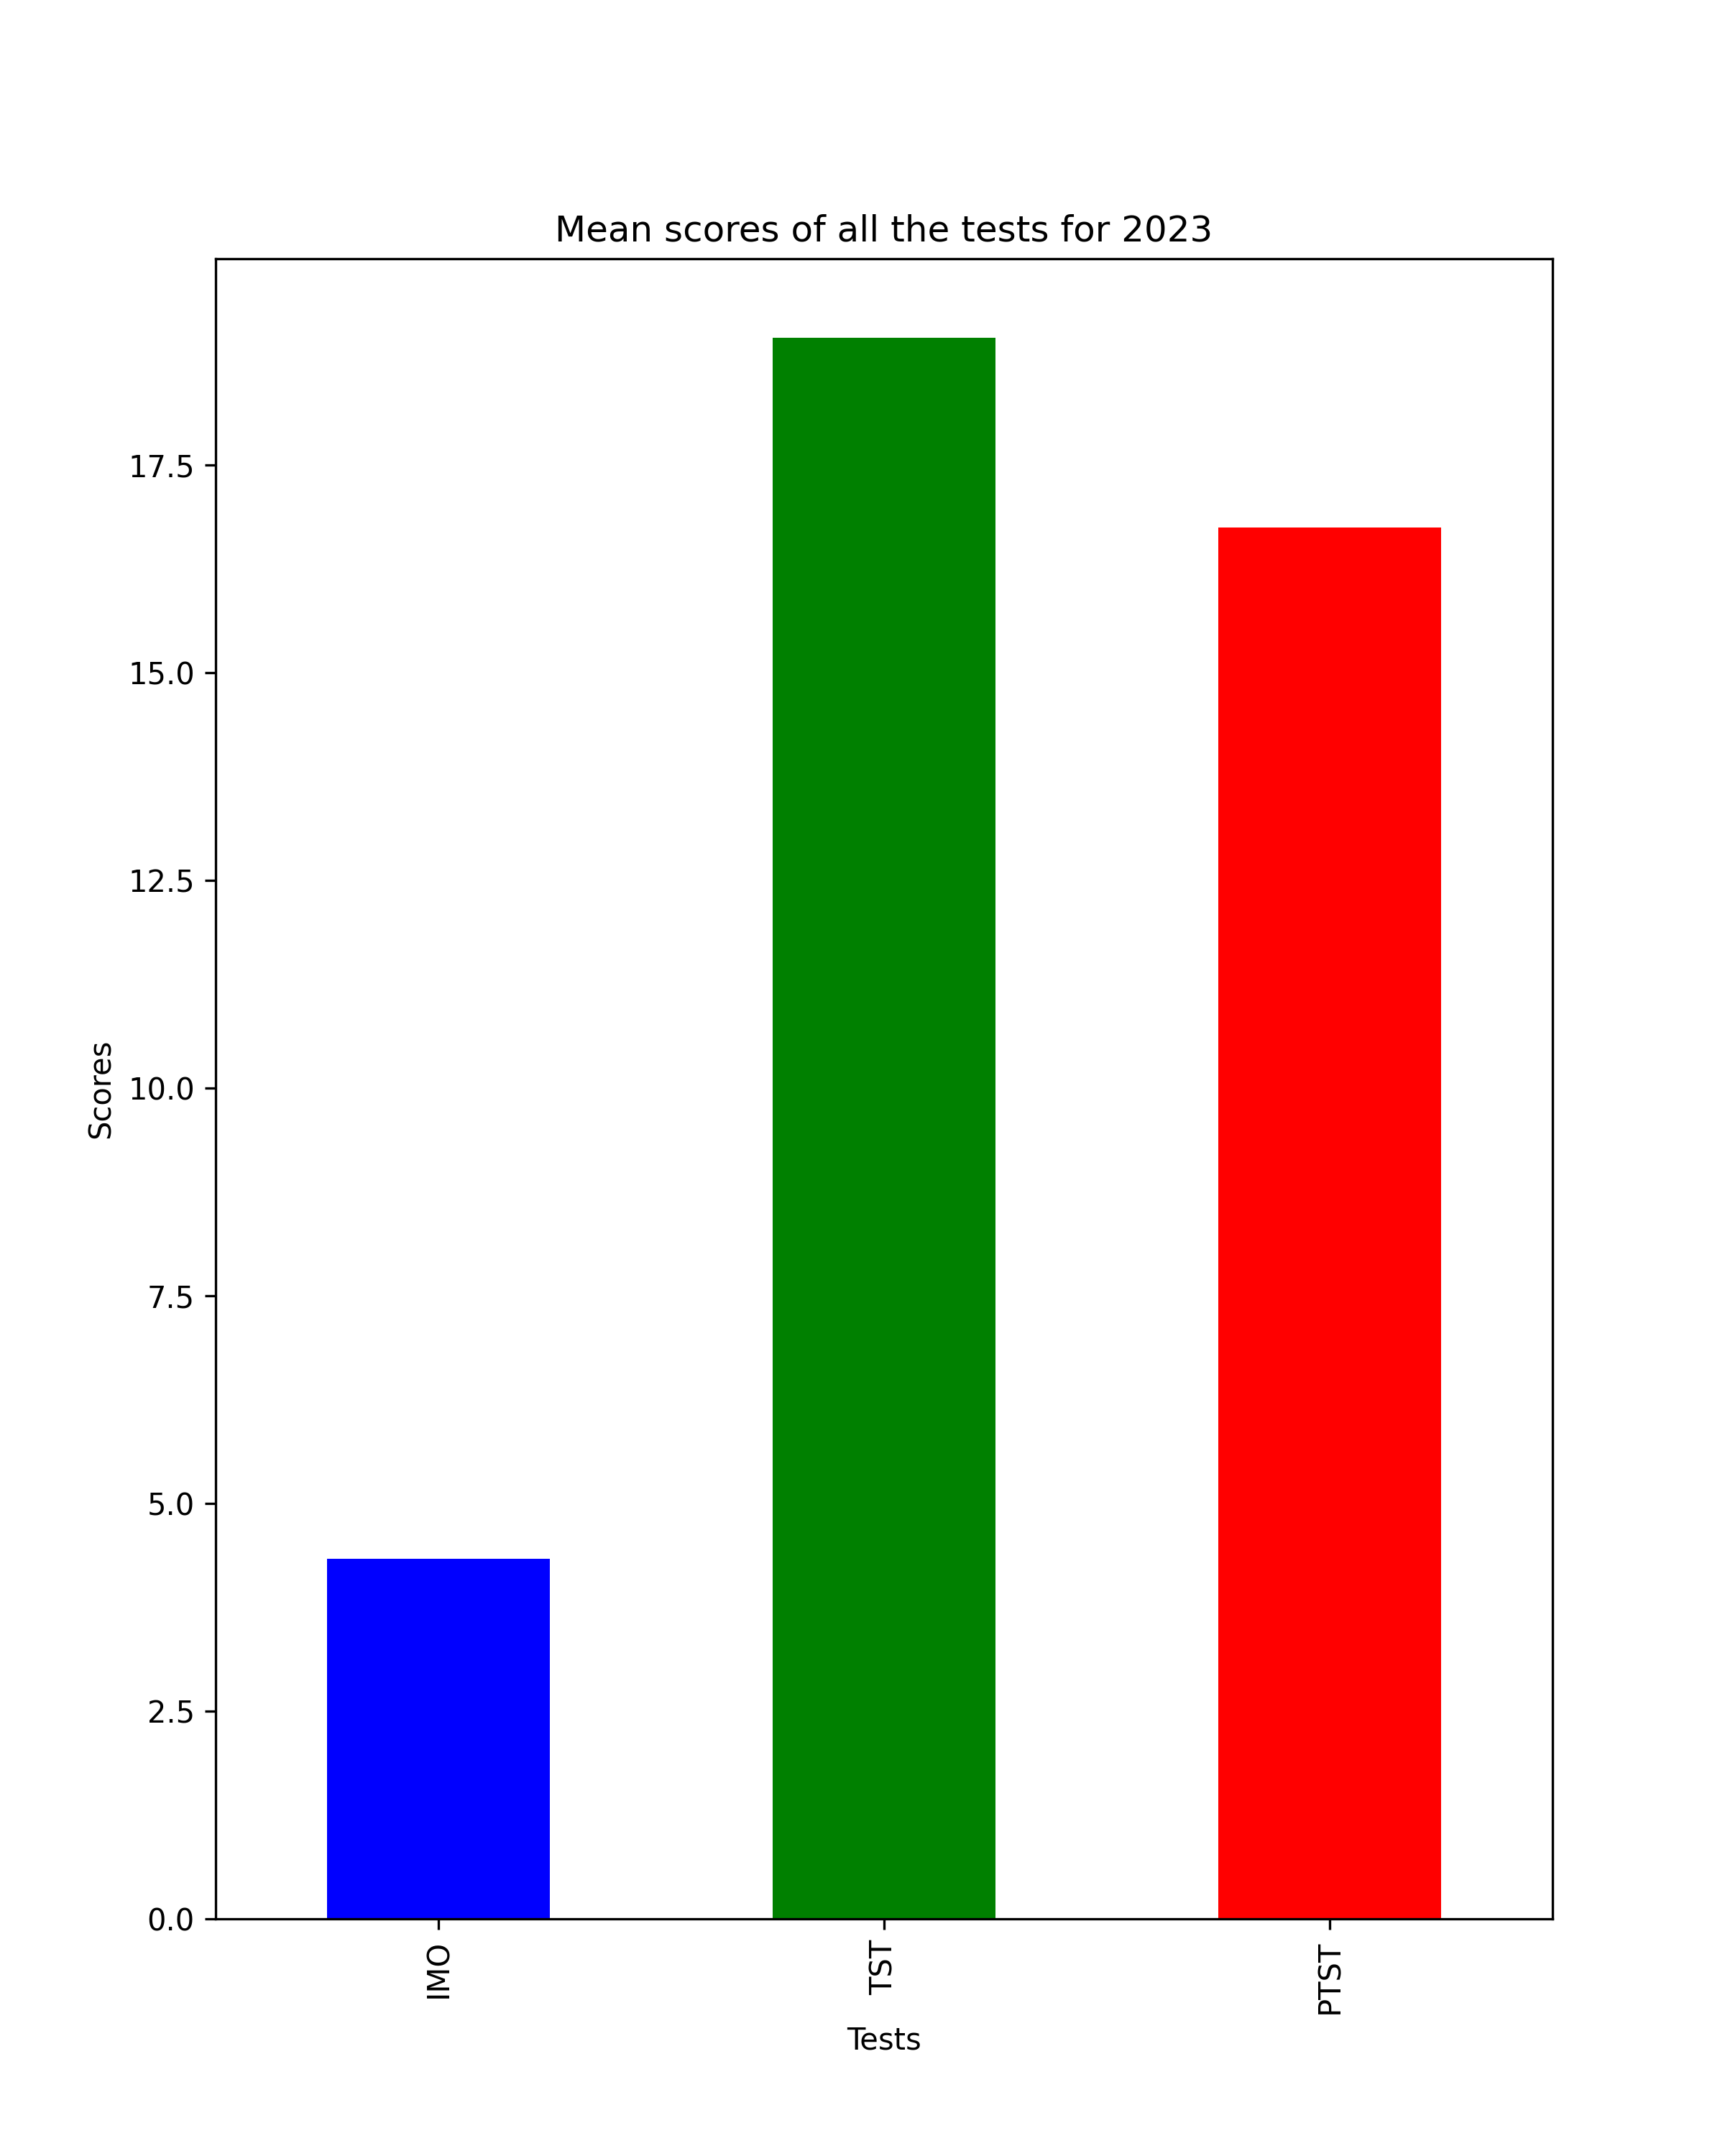
\includegraphics[width=0.5\textwidth]{2023_mean.png}
    \caption{Mean scores across IMO, TST, and PTST for the year 2023.}
    \label{fig4}
\end{figure}

\begin{figure}[H]
    \centering
    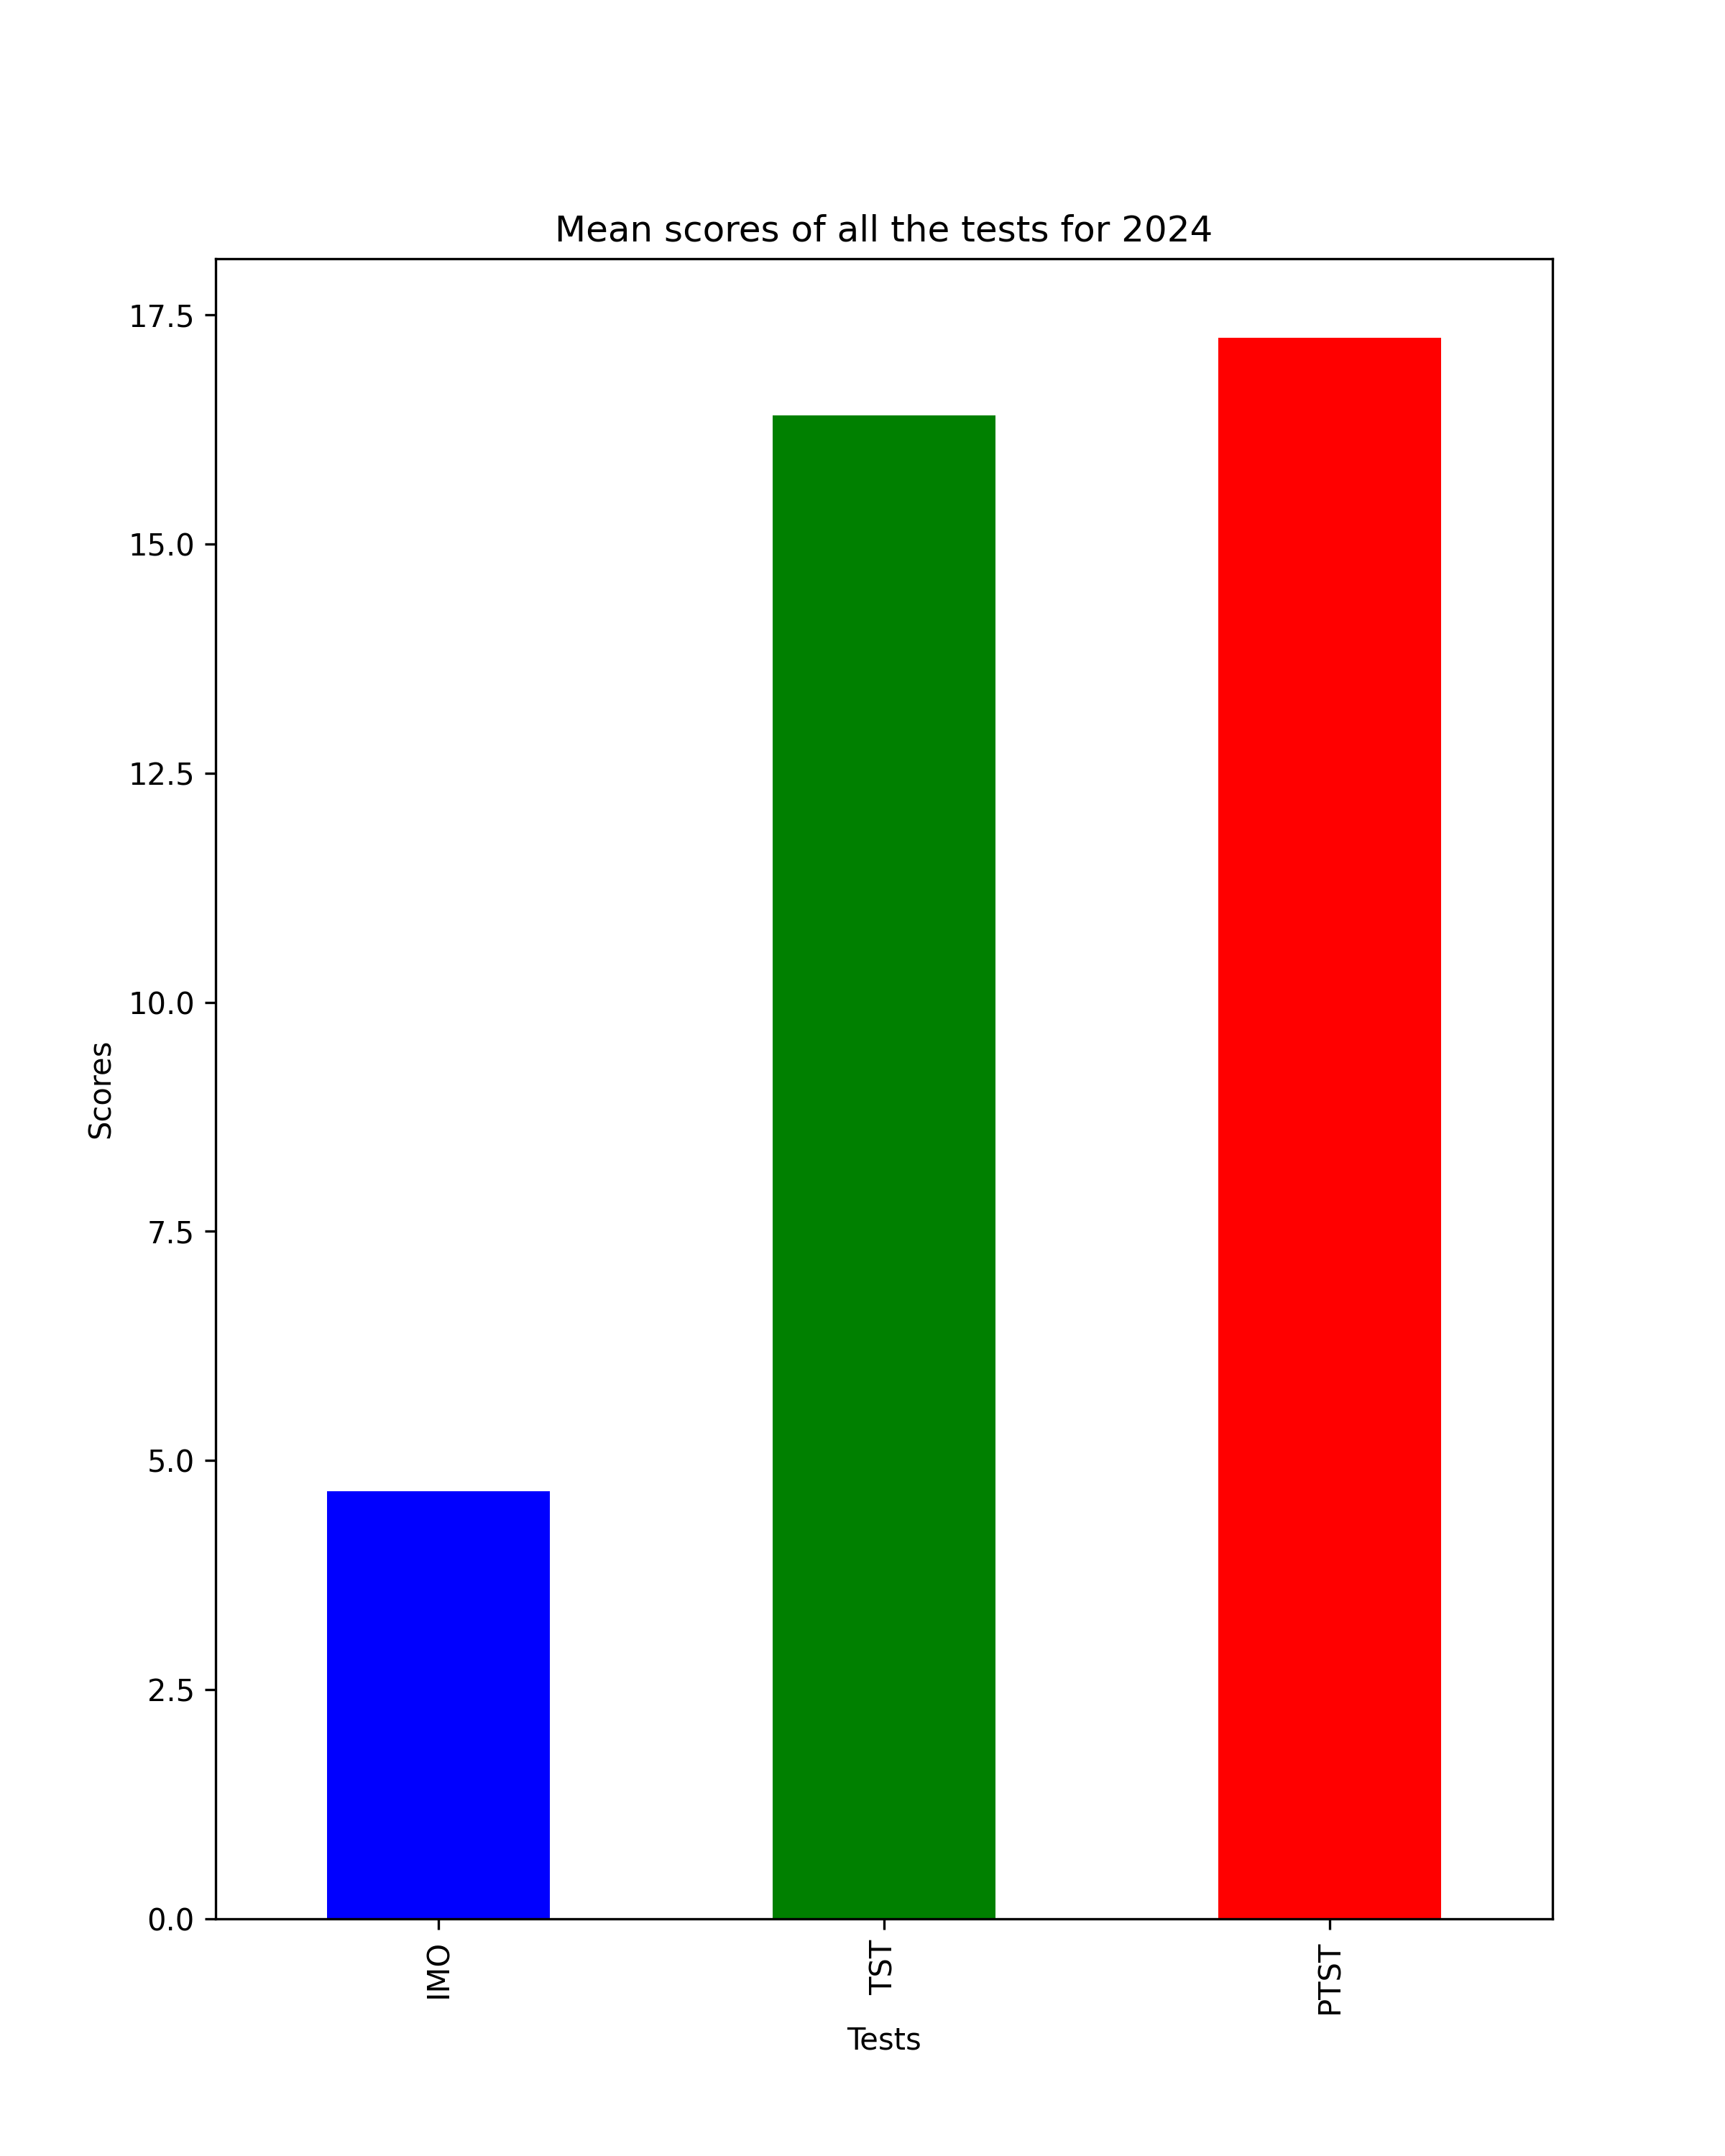
\includegraphics[width=0.5\textwidth]{2024_mean.png}
    \caption{Mean scores across IMO, TST, and PTST for the year 2024.}
    \label{fig5}
\end{figure}

\begin{figure}[H]
    \centering
    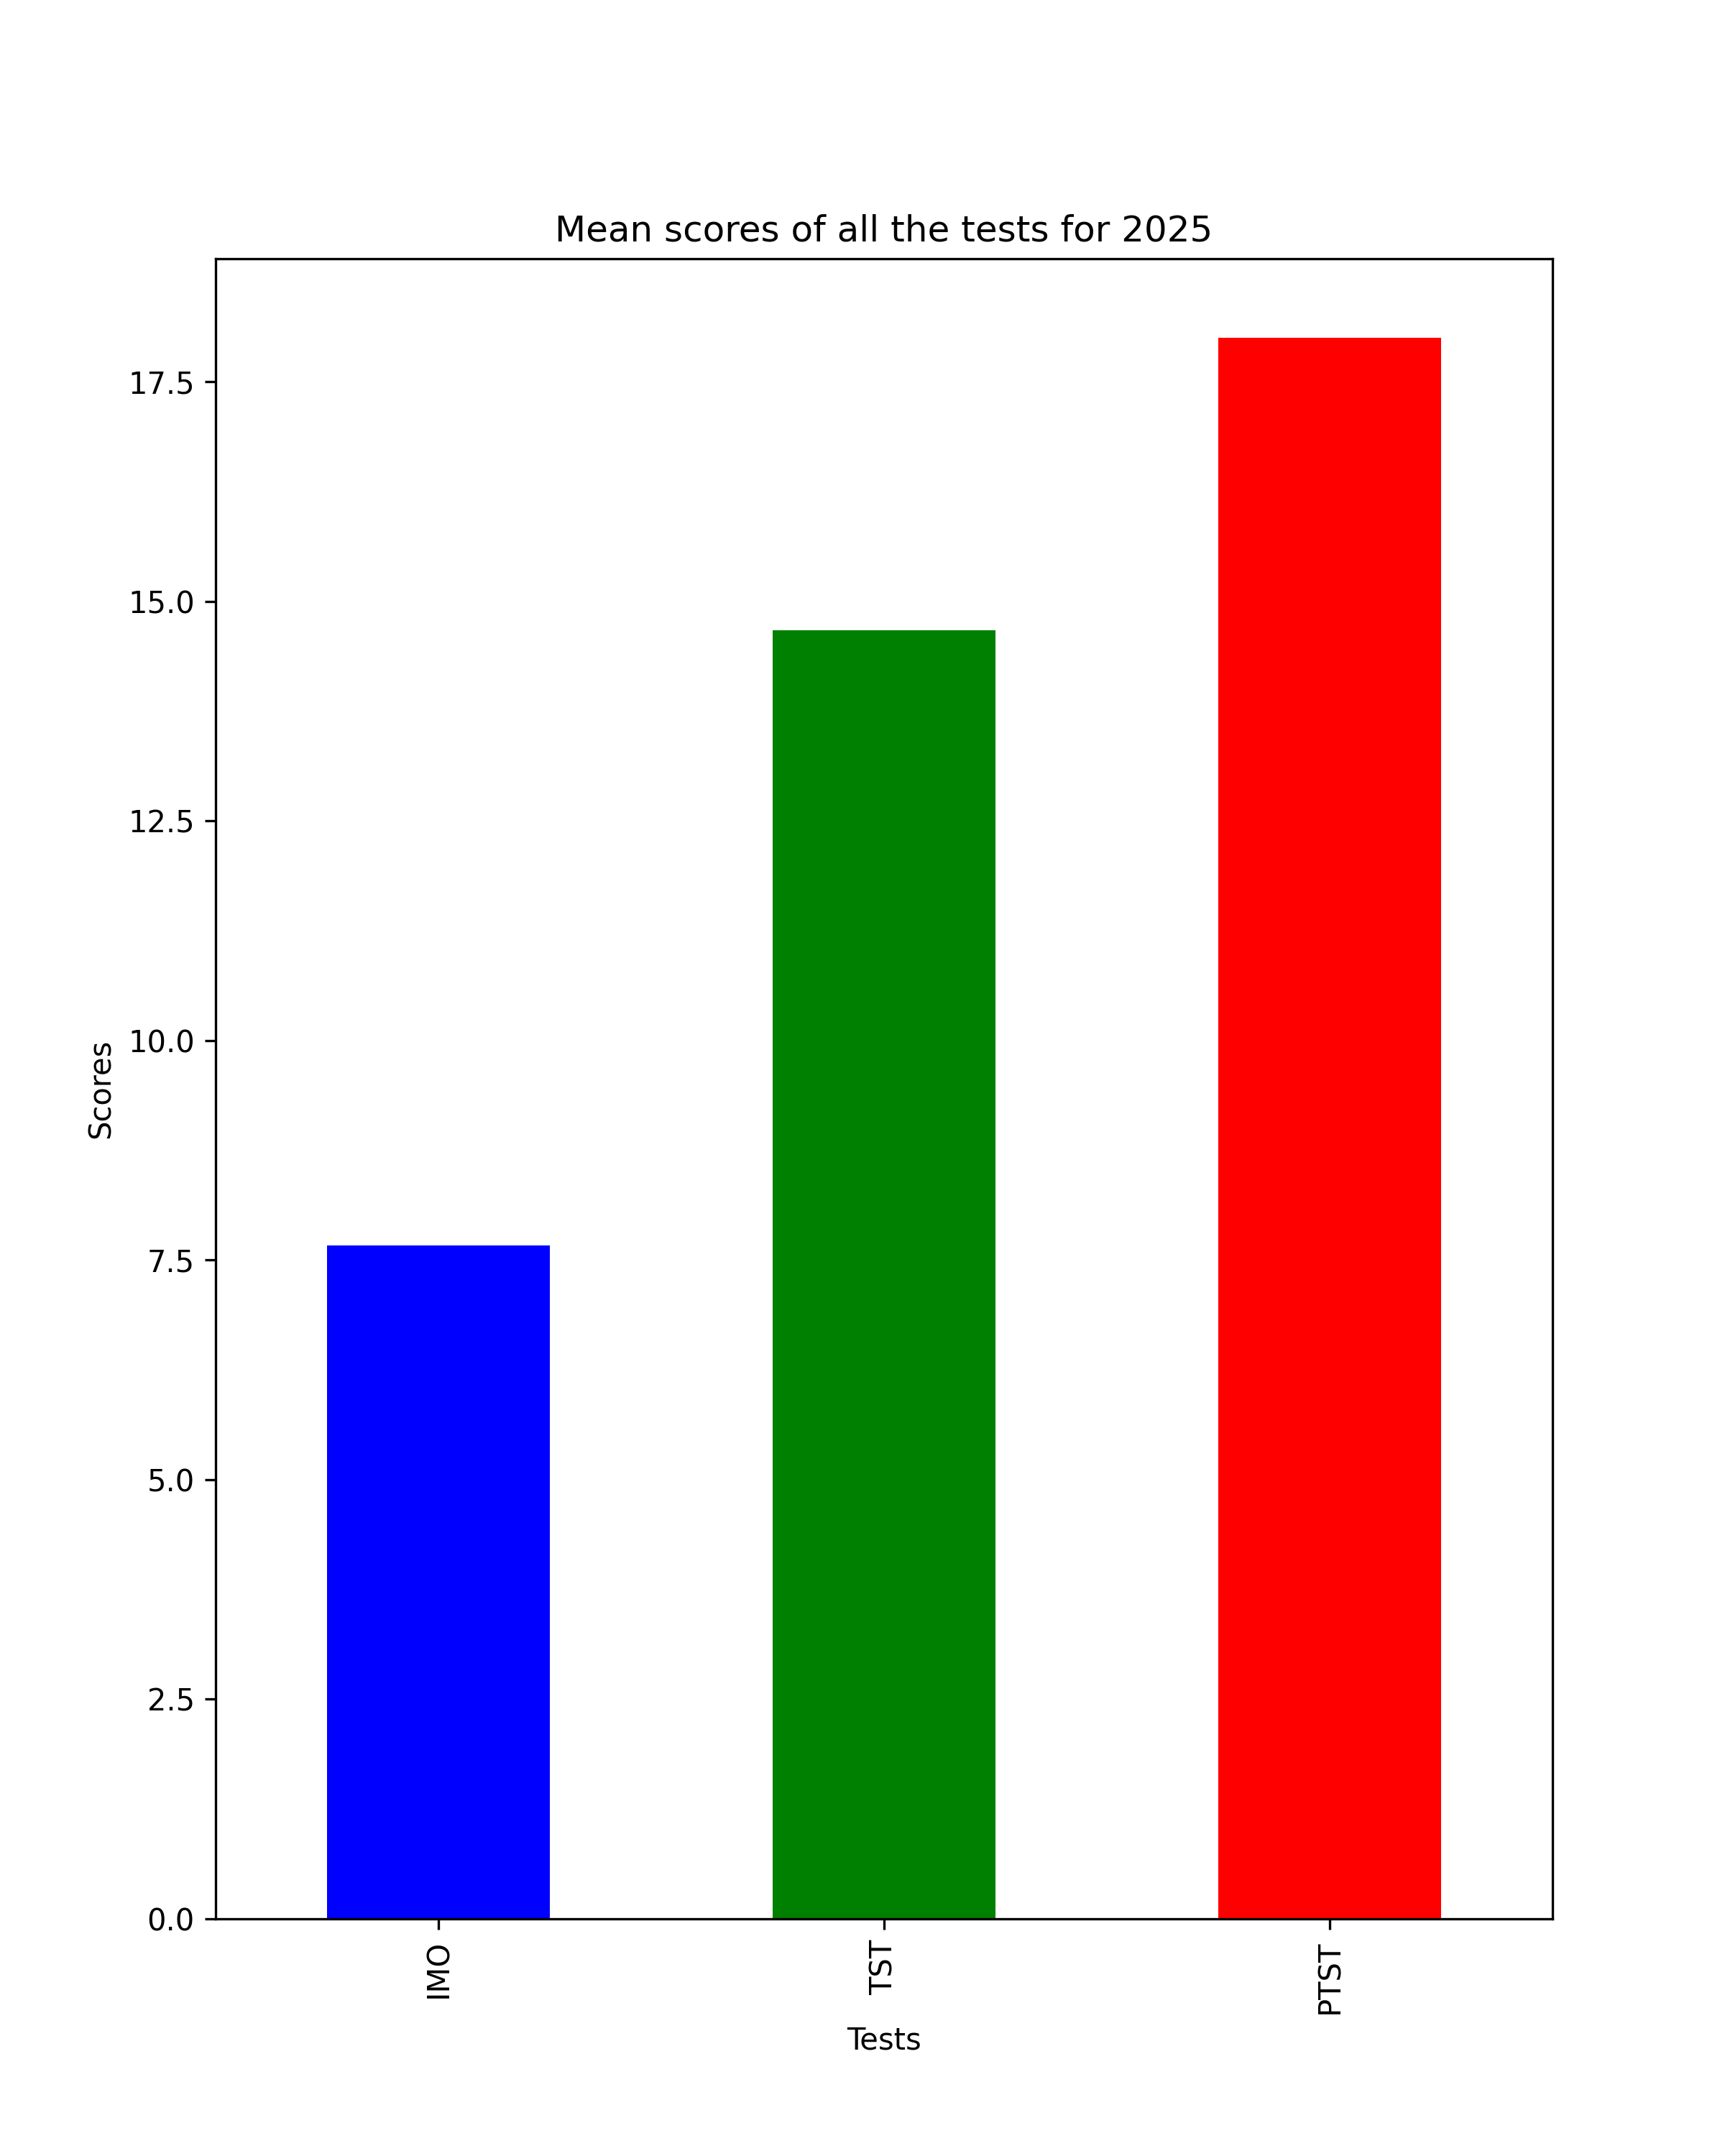
\includegraphics[width=0.5\textwidth]{2025_mean.png}
    \caption{Mean scores across IMO, TST, and PTST for the year 2025.}
    \label{fig6}
\end{figure}
\newpage

The mean scores for all three data sets(2023, 2024 and 2025) reveal similar average score for PTST and TST across all three years. In 2023, the TST mean is marginally higher than the PTST mean. This reversed in 2024 and 2025 where PTST mean is just slightly higher than TST mean. Another pattern that can be seen is that there is a large and consistent gap between average scores of both the internal tests and IMO (The internal testing average ranges from 15-19 while the IMO average ranges from 4-8, which makes the ratio between the tests and IMO nearly 1:4).

These data indicates that the internal tests are easier than the IMO. This observation alongside the P1/P4 growth suggests that the internal tests seem to particularly focus on P1/P4 level.

However, despite the mean scores being similar, we cannot conclude that two tests, TST and PTST are so similar difficulty level. To understand the true character of each test, it is necessary to examine the standard deviation across two tests. 

\begin{figure}[H]
    \centering
    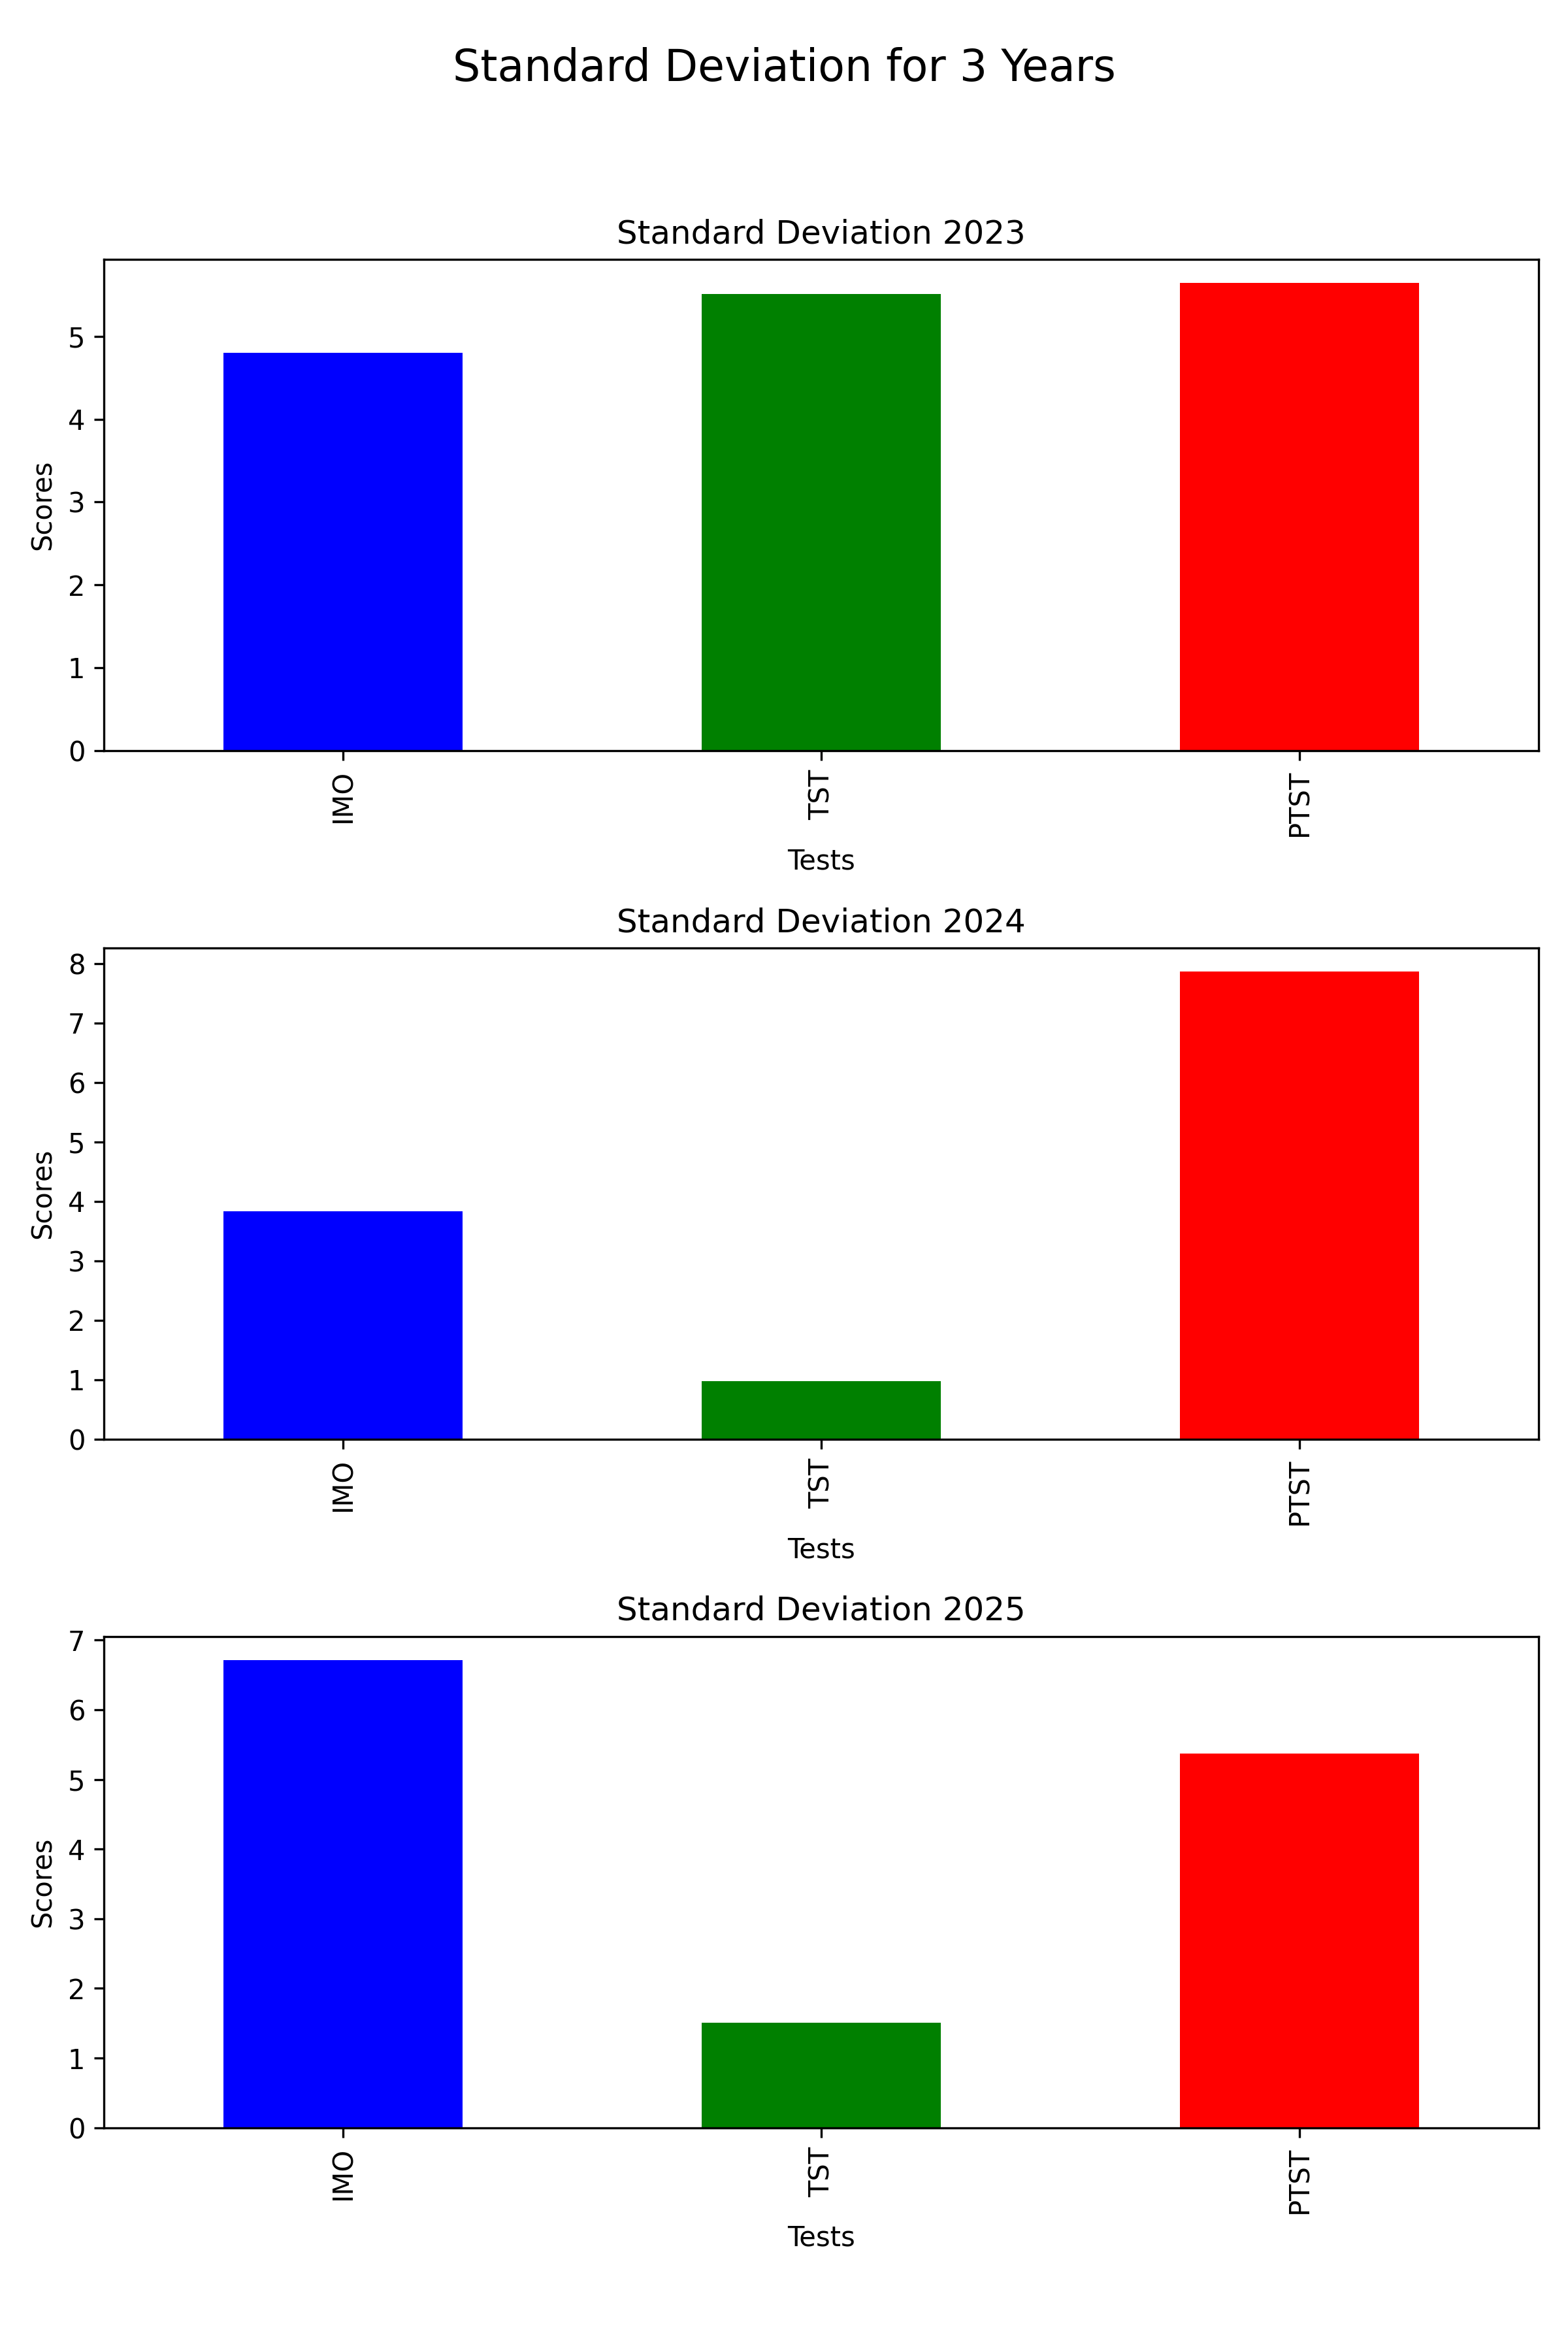
\includegraphics[width=0.6\textwidth]{standard_deviation.png}
    \caption{Standard deviation across tests(IMO, TST and PTST) for years 2023, 2024 and 2025.}
    \label{fig7}
\end{figure}
\newpage
The following things can be noticed through the standard deviation graphs:

\begin{itemize}
    \item[i)] The TST has low standard deviation (near 0) for years 2024 and 2025. This suggests that the 6 people who went to IMO scored in similar ranges (in TST) due to which their scores didn't fluctuate a lot from each other. All students seem to be performing on similar questions while being blocked by harder ones.
    \item[ii)] The PTST has very high standard deviation, with 7.9 as the highest in 2024. This suggests that the PTST scores are widely spread, far more than TST scores. However, despite showing spread similar to IMO, the test doesn’t model IMO. Later in Section 0.4 we find that this scatter is majorly influenced by presence of outliers.
    \item[iii)] The standard deviation for IMO sits between deviation for TST and PTST. The three-year data shows that the scores remain spread in the competition.
\end{itemize}

Among these observations, the TST standard deviation hovering around 0-1 strengthens the argument made regarding focus on P1/P4 problems identified in previous section. When six candidates are just separated by a single point, it reveals that the test may lack discriminatory power to separate between candidates. This can majorly be due to focus of extremes where majority of the questions are P1/P4 level (as evidenced by the mean) and some of the questions are in P3/P6 level (on two side of extremes). 

The high standard deviation for PTST is also an observation to be noted. While it may seem that PTST brings more spread to data which helps distinguish real performers, the reality seems to be quite different. From two previous sections it can be seen that one or two students perform exceptionally in PTST in questions setting which doesn't quite reflect the IMO environment. This is further evidenced in next section where three scatter plots are used to show how candidates perform different tests.

\subsection{Scatter Analysis of Internal and International Tests}
Figure \ref{fig8}, \ref{fig9} and \ref{fig10} present scatter plots from the year 2023, 2024 and 2025 respectively. Each blue plot represents a student's PTST scores (in x axis) compared to the IMO scores (in the y axis), and each orange plot represents a student's TST scores (in x axis) compared to the IMO scores (in the y axis). Gray lines connect the two internal scores for each individual, visually suggesting the change between two test stages.

\begin{figure}[H]
    \centering
    \includegraphics[width=0.6\textwidth]{2023_compare.png}
    \caption{Internal vs External score comparison for year 2023. IMO score (Y axis) plotted against PTST scores (blue) and TST scores (orange).}
    \label{fig8}
\end{figure}

The scatter plot for 2023 (Figure \ref{fig8}) reveals clustered distribution. This clustering at IMO score = 2 is primarily a consequence of students solving one problem partially. The numerical data for PTST and TST far off from the scores achieved by candidates in IMO. The individual with the highest score (14 in IMO) can be clearly seen as an outlier whose performance has disproportionately high as compared to other candidates. This is due to the prodigy effect.

While both TST and PTST was accurately able to predict this high performer (on the right side of the graph), they failed to differentiate between other performers, all of whom scored significantly low in IMO regardless of their rank.

\begin{figure}[H]
    \centering
    \includegraphics[width=0.6\textwidth]{2024_compare.png}
    \caption{Internal vs External score comparison for year 2024. IMO score (Y axis) plotted against PTST scores (blue) and TST scores (orange).}
    \label{fig9}
\end{figure}

The Figure \ref{fig9} provides evidence for claim stated in Section 0.4 where it was stated that despite high standard deviation of PTST, it doesn't accurately model IMO environment. In this scatter plot we can see that the individual who scored significantly high (around 34 points) in PTST examinations was able to secure only 3 marks in IMO. Meanwhile a student with lower PTST score was able to secure 11 marks in the IMO. This shows that despite having high spread the PTST doesn't seem to be modelling IMO. It can also be seen that while numerically both significantly overestimate IMO performance, TST out of the two predicts the relative rankings among the candidates better. 

\begin{figure}[H]
    \centering
    \includegraphics[width=0.6\textwidth]{2025_compare.png}
    \caption{Internal vs External score comparison for year 2025. IMO score (Y axis) plotted against PTST scores (blue) and TST scores (orange).}
    \label{fig10}
\end{figure}

The 2025 scatter (Figure \ref{fig10}) contains the most scattered scores ranging from 2 to 20. Moreover, the predictive ranking of TST is mostly preserved, with a few expected inconsistencies, and the TST comes up to be the better predictor among internal two tests in terms of relative rankings. This pattern largely visible in year 2024 and 2025 is the principle finding of this section.

Neither PTST nor TST accurately predicts the numerical score a candidate is likely to get in IMO. However, TST among the two was a better predictor of relative performance rankings than PTST. This is not because TST is more sophisticated as it is already evidenced in Section 0.4.3 that the test has minimal standard deviation. This is likely is because the TST's compressed environment filtered out the PTST outliers due to which it could produce more stable ranking, even if the score differences (standard deviation) for the data were low. 

Key insights: It is suggested by the data that TST predicts relative rankings and possible IMO trends better than PTST, due to its compressed environment where outliers, as seen in PTST. However, this is a hypothesis as only 3 years of data is involved and shouldn’t be termed as final conclusion.

\subsection{Synthesis of Findings}
The data examined above under 0.4 sections provide a decently clear picture of Nepal's journey in IMO with minor nuances. While the growth of Nepal as an IMO participant is clearly visible, the growth mostly seems to come from P1/P4 problems, problems which lie in the easier side of the spectrum. This seems to be happening because the institutions are likely prioritizing selection and practice focused on skillset required for solving these problems.

The PTST has more differentiation and spread in its data, but this spread is largely due to one or two performers who end up getting high outlier scores. The fact that PTST scores cannot be termed more relevant is because of the inconsistency it provides. The higher scorer in PTST sometimes ends up scoring very low in IMO and vice versa. The 2024 scatter plot is the clearest evidence of this failure.

The TST, on the other hand, despite having similar average scores to PTST seems to be working on different model as is evidenced by its low standard deviation in 2024 and 2025.

\section{Recommendations}

\subsection{Shift in Internal Testing towards P2/P5 questions}
Throughout the paper it has been evidenced that the current testing system primarily seems to focus on testing students on the basis of P1/P4 questions, which in fact has brought positive results in IMO with rapidly growing total scores. However, if the testing system continues the scores are likely to approach a plateau. To continue this upward trend of development it is recommended to shift towards P2/P5 questions which will likely result in reduced outlier and act as a bridge between the ceiling and growth. 

\subsection{Raise the difficulty floor from lower levels}
While the above suggestion could be carried out, the significant change may take time if the testing difficulty isn't slowly raised from lower levels. When P2/P5 type questions are only focused in later stages (PTST or TST ) then a shock is likely to appear between students and the scores can drop. So, it is recommended that the changes are made from lower curriculum itself. 
\newpage
\section{Conclusion}
\begin{enumerate}
    \item Nepal is developing at rapid rate, with year each accumulating higher cumulative marks than the year before. However, this development seems to be driven by mastery of P1/P4 (easy level problems). P3/P6 questions have been never solved (1 point in 9 years), and the P2/P5 questions show fluctuated improvement with no real growth. 
    \item The average scores between IMO and internal tests show a huge gap (internal scores are very high), even for a nation who has recently joined IMO and are yet to finalize the testing system (The ratio between mean of internal tests and IMO is around 1:4). This is likely due to prioritization of P1/P4 type of problems.
    \item The exceptional growth that Nepal is having is likely to slow down if the P1/P4 prioritization is truly focused, and the marks are likely that performance may approach a plateau under current conditions. The inclusion of P2/P5 problems as a buffer and bridge can avoid this.
\end{enumerate}

\newpage
\section*{References}
Mathematical Association of Nepal. (2023). National Level Mathematical Olympiad Results 2023/024. \\
Mathematical Association of Nepal. (2024). National Level Mathematical Olympiad (Pre-TST and TST) Results 2080. \\
Mathematical Association of Nepal. (2025). National Level Mathematical Olympiad (NMO 2024/025-TST) Results 2081. \\
International Mathematical Olympiad. (2017–2025). Country individual results: Nepal. Retrieved from their website.

\end{document}